\chapter{Quantencomputer\label{chapter:quantencomputer}}
\lhead{Quantencomputer}
\rhead{}
Die Technologie des zwanzigsten Jahrhunderts hat automatische
Rechenmaschinen hervorgebracht, beliebige Rechnung durchf"uhren,
sofern sie die Speichergr"osse der Maschine nicht sprengen.
Sie beruhen auf einer physischen Codierung der Zahlen, mit denen
gerechnet werden soll, und einer Maschine, welche Codierungen 
in neue Codierungen umwandelt.
\index{Babbage, Charles}
Die Idee einer solchen Maschine geht auf Charles Babbage zur"uck,
der in den Jahren ab 1812 auch eine Realisierung als mechanische
Maschine angestrebt hat.

Moderne Computer sind alle konkrete Realsierungen des abstrakten
\index{Turing, Alan}
Konzeptes der Turing-Ma\-schi\-ne, welches Alan Turing formuliert hat,
um zu analysieren, welche Arten von Berechnungen in welcher Zeit
"uberhaupt durchgef"uhrt werden k"onnen.
Es wurde erkannt, dass gewisse Probleme auf Turing-Maschinen
derart lange ben"otigen w"urden, dass man sie getrost als undurchf"uhrbar
betrachten kann.
\index{Faktorisierung}
Allgemein besteht die "Uberzeugung, dass das Problem der Faktorisierung
des Produktes von grossen Primzahlen in diese Kategorie geh"ort,
auch wenn dies bisher nicht bewiesen worden konnte.
Dies impliziert, dass eine solche Faktorisierung, auf der die Sicherheit
verschiedener kryptographischer Systeme basiert, ohne zus"atzliches
Wissen nicht durchf"uhrbar ist.

Eine wesentliche Eigenschaft solcher schwieriger Problem ist, dass
sie die parallel Evaluation sehr vieler M"oglichkeiten erfordern,
was in einem klassischen Computer nur sequenziell m"oglich ist.
Der Grund daf"ur ist, dass ein Bit immer nur in genau einem
Zustand sein kann, wenn man die verschiedenen M"oglichkeiten des
Bits evaluieren will, dann muss man das hintereinander tun.

In der Quantenmechanik gibt es aber Systeme, die in zwei Zust"anden
gleichzeitig sein k"onnen, wie wir im Abschnitt~\ref{section:cat}
illustrieren werden.
Wenn man also auch das Rechenwerk einer Turingmaschine durch eine
``Quantenschaltung'' ersetzen kann, dann kann ein relativ kleiner
Quantencomputer alle M"oglichkeiten aller Bits gleichzeitig evaluieren,
und damit das Problem in sehr kurzer Zeit l"osen.

\section{Klassische Computer}
\rhead{Klassische Computer}
\index{Computer!klassischer}
\index{Gatter!logisches}
Ein klassischer Computer kann bin"ar als Spannungen in einer
elektronischen Schaltung codierte Zahlen in ander Muster von
Spannungen umwandeln, welche das Resultat einer Rechenoperation
mit den Zahlen als Input darstellt.
\begin{figure}
\centering
\begin{tabular}{cccc}
&UND&ODER&XOR\\
\\
&
\includegraphics{graphics/gatter-1.pdf}&%
\includegraphics{graphics/gatter-2.pdf}&%
\includegraphics{graphics/gatter-5.pdf}
\\
\\
&
\includegraphics{graphics/gatter-3.pdf}&%
\includegraphics{graphics/gatter-4.pdf}&%
\includegraphics{graphics/gatter-6.pdf}
\end{tabular}
\caption{Logische Gatter von links nach rechts UND, ODER, XOR,
in der unteren Reihe invertiert.
\label{skript:gates}}
\end{figure}
\index{Halbaddierer}
\index{Volladdierer}
Die grundlegenden logischen Operationen werden dann durch sogenannte
Gatter implementiert, deren Schaltbilder in Abbildung~\ref{skript:gates} dargestellt
sind.
\begin{figure}
\centering
\includegraphics{graphics/gatter-8.pdf}
\caption{Halbaddierer, der Ausgang $\Sigma$ ist die Summe der beiden
Eing"ange $A$ und $B$, der Ausgang $C_\text{out}$ wird aktiv, wenn
ein "Ubertrag auftritt.
\label{skript:halfadder}}
\end{figure}
\begin{figure}
\centering
\includegraphics{graphics/gatter-7.pdf}
\caption{Volladdierer, berechnet die Summe der beiden Inputs $A$ und $B$
und den "Ubertrag $C_\text{in}$, und gibt die Summe $\Sigma$ und den
"Ubertrag $C_\text{out}$ aus.
\label{skript:fulladder}}
\end{figure}
Aus den Grundoperationen lassen sich komplexere Schaltungen 
aufbauen, zum Beispiel das Halbaddierwerk in Abbildung~\ref{skript:halfadder}
oder der Volladdierer in Abbildung~\ref{skript:fulladder}.
Die Digitaltechnik lehrt, wie man durch Kombination solcher Schaltung
beliebig komplexe Berechnungen anstellen kann.

Die Verbindungen in all diesen Schaltungen k"onnen nur in jeweils einem
Zustand sein, ein oder aus, $1$ oder $0$.
Dies ist eine Einschr"ankung der Technologie.
Selbst die Verwendung verschiedener Spannungsniveaus auf den Verbindungen
w"urde daran nichts "andern: zu jeder Zeit kann jede Verbindung nur
ein einem der m"oglichen Zust"ande sein.

\index{SAT}
Eines der schwierig zu l"osenden Probleme ist SAT, die Frage, ob eine
logische Formel durch geeignete Wahrheitsbelegung der Inputs wahr
werden kann. Implementiert man die logische Formal als Schaltung,
wird die Frage gleichbedeutend damit, ob der Ausgang der Schaltung
durch geeignete Beschaltung der Inputs in den Zustand $1$  gehen kann.
Bedingt durch die Technologie k"onnen wir die Frage nur dadurch beantworten,
dass wir alle m"oglichen Inputs durchprobieren. Bei $n$ Inputs sind
dies $2^n$ Belegungen, entsprechend lange dauert es, eine L"osung
zu finden.

\section{Schr"odingers Katze\label{section:cat}}
\rhead{Schr"odingers Katze}
\index{Katze!Schr\"odinger}
\begin{figure}
\centering
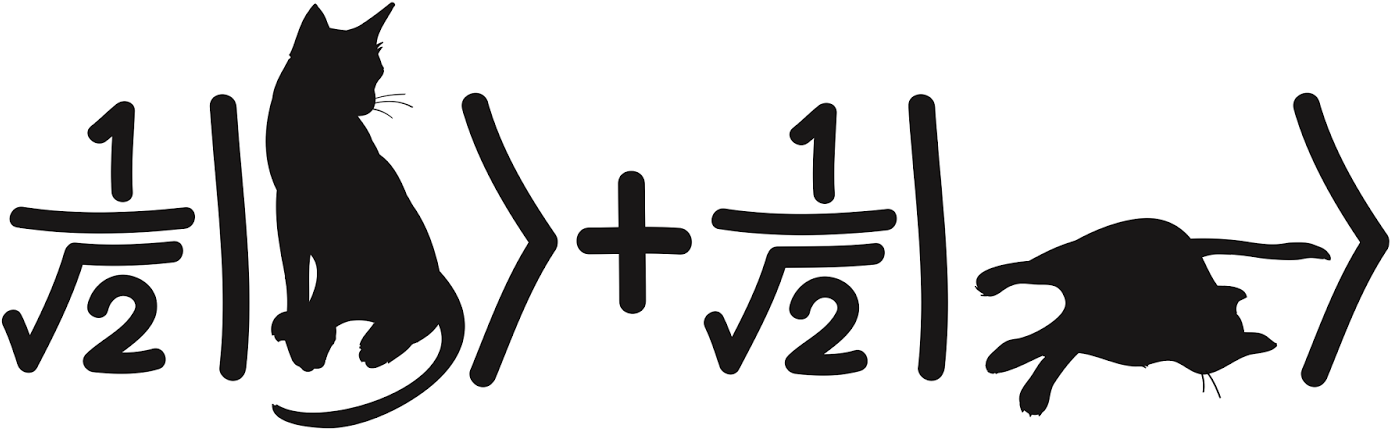
\includegraphics[width=0.5\hsize]{images/catliveanddead2.png}
\caption{Schr"odingersche Katze in einem "Uberlagerungszustand
\label{skript:deadandalive}}
\end{figure}
Dass in der Quantenmechanik ein System nicht in einem reinen Zustand
zu sein braucht, hat Erwin Schr"odinger mit seinem ber"uhmten 
Gedankenexperiment mit der Katze illustriert.
In einer Kiste befindet sich eine Katze und ein Mechanismus,
der beim radioaktiven Zerfall des darin befindlichen radioaktiven
Atomkernes eine Phiole mit Gift zerbricht, so dass es entweichen und
die Katze t"oten kann.
Die Katze kann offensichtlich in zwei m"oglichen Zust"anden sein,
lebendig $|\smiley\rangle$ oder tot $|\frownie\rangle$. 
Zu beginn des Experiments befindet es sich im Zustand $|\smiley\rangle$.
Dieser Zustand der Katze wiederspiegelt nat"urlich nur den Zustand
des Atomkerns, der ebenfalls in zwei Zust"anden sein kann.

Mit fortschreitender Zeit steigt die Wahrscheinlichkeit, dass der
Atomkern zerfallen ist, und die Katze tot ist.
Genauer sind die Wahrscheinlichtkeiten, die Katze in den beiden
Zust"anden zu finden
\begin{align*}
|\langle \smiley|\psi(t)\rangle|^2
&=
2^{-t/t_{\frac12}}
&&\text{und}
&
|\langle \frownie|\psi(t)\rangle|^2
&=
1-2^{-t/t_{\frac12}}
\end{align*}
Die Katze ist also in einem Zustand
\[
|\psi(t)\rangle = 
\sqrt{2^{-t/t_{\frac12}}}e^{i\varphi_1(t)}\,|\smiley\rangle
+
\sqrt{1-2^{-t/t_{\frac12}}}e^{i\varphi_2(t)}\,|\frownie\rangle,
\]
die beiden Phasenfaktoren tragen der Tatsache Rechnung, dass komplexe
Linearkombinationen m"oglich sind (Abbildung~\ref{skript:deadandalive}).

Ist die Katze lebendig oder tot? Die Erfahrung mit makroskopischen
Katzen sagt uns, dass ein Katze entweder das eine oder andere ist.
Die Quantenmechanik sagt uns dagegen, dass wir es nicht wissen k"onnen.
Wir k"onnen nur wissen, dass die Katze in einem "Uberlagerungszustand
ist.
Das einzige, was wir daraus ableiten k"onnen, ist mit welcher
Wahrscheinlichkeit sie bereits tot ist.
Gewissheit dar"uber, in welchem Zustand sich die Katze befindet,
erhalten wir genau in dem Moment, wo wir das Experiment durchf"uhren
und den Zustand der Katze ermitteln.

Durch den Prozess der Beobachtung der Katze "andert sich deren Zustand.
Lebt sie noch, wissen wir, dass sie sich im Zustand $|\smiley\rangle$ befindet.
Ist sie tot, befindet sie sich im Zustand $|\frownie\rangle$.
Die Beobachtung hat also den Zustand ver"andert.

Wir erweitern jetzt das urspr"ungliche Gedankenexperiment von Schr"odinger.
Wir stellen uns vor, wir m"ochten gerne eine exotische Eigenschaft von
Katzen messen, insbesondere m"ochten wir wissen ob eine lebende Katze oder
eine tote Katze diese Eigenschaft hat. Das klassische Experiment
daf"ur w"are, je eine lebendige und eine tote Katze zu pr"aparieren,
und dann den Test f"ur die Eigenschaft auf beide anzuwenden.

F"ur das quantenmechanische Experiment brauchen wir offenbar einen
Operator $Q$ (f"ur ``question''), der zwei m"ogliche Ausgangszust"ande hat:
die Katze mit der
Eigenschaft $|Y\rangle$ und die Katze ohne die Eigenschaft $|N\rangle$.
Das zugeh"orige Experiment k"onnte man mit der Notation aus
Kapitel~\ref{chapter:einfache-quantensysteme} als
\begin{center}
\includegraphics{graphics/gatter-9.pdf}
\end{center}
darstellen. 

F"ur Schr"odingers Katze k"onnen wir die Frage, ob die Eigenschaft $Q$
in f"ur lebende oder tote Katzen vorhanden ist, in einem einzigen
Durchgang beantworten.
Dazu stellen wir zuerst eine Katze in einem "Uberlagerungszustand
$|\psi\rangle$ von $|\smiley\rangle$ und $|\frownie\rangle$ her\footnote{
Man beachte, dass dies nicht bedeutet, dass die H"alfte der so pr"aparierten
Katzen leben und die anderen tot sind.
Vielmehr befindet sich die Katze in beiden Zust"anden, erst bei der
Messung wird festgelegt, was der in dieser Durchf"uhrung des Experimentes
gemessene Zustand ist.
}.
Auf diesen Zustand wenden wir den Operator $Q$ an, und testen dann,
ob es Katzen gibt, die sich im Zustand $|Y\rangle$ befindet, indem
wir $\langle Y|\,Q\,|\psi\rangle$ messen.
Falls wir herausfinden, dass $\langle Y|\,Q\,|\psi\rangle\ne 0$,
dann kann eine Katze die Eigenschaft haben, auch wenn wir noch nicht
wissen, ob es eine Eigenschaft von toten oder lebenden Katzen ist.

Schr"odingers Katze in ihrem "Uberlagerungszustand kann also dazu
verwendet werden, einen Quantencomputer zu bauen, der Probleme "uber
Katzeneigenschaften l"osen kann.
Im Gegensatz zu einem klassischen Computer k"onnen wir aber nicht
erwarten, dass wir in einer einzigen Messung das Resultat der
Berechnung bekommen k"onnen.
Das Quantensystem kann nur eine Wahrscheinlichkeitsaussage liefern,
und Messungen der Wahrscheinlichkeit verlangen immer eine grosse Zahl
von Experimenten.

Ein praktisch n"utzlicher Quantencomputer muss noch weit gr"ossere
Qubits realisieren.
Ein Quantencomputer mit $n$ Qubits ist in der Lage, einen Zustand
herzustellen, in dem $2^n$ Zust"ande "uberlagert sind. 

\section{Probabilistische Algorithmen}
\rhead{Probabilistische Algorithmen}
\index{Algorithmus!probablistischer}
Bis jetzt ist klar, dass wir von einem Quantencomputer keine definitiven
Antworten erhalten k"onnen, sondern nur Aussagen "uber Wahrscheinlichkeiten.
Dies ist aber nicht wirklich etwas Neues, denn schon lange werden
zum Beispiel in der Kryptographie Algorithmen verwendet, die ebenfalls
nur probabilistische Aussagen machen.
Wenn man eine RSA Schl"usselpaar f"ur ein X.509-Zertifikat erzeugen will,
muss testen, ob eine mehrere Tausend Bit lange Zahl $n$ eine Primzahl ist.
Es w"urde viel zu lange dauern, die Primzahleigenschaft durch Testdivision 
zu ermitteln.
Zwar ist inzwischen ein Algorithmus mit polynomieller Laufzeit
bekannt \cite{skript:aks}, trotzdem
verwendet man meistens einen probabilistischen Test, der nur mit einer
gewissen Wahrscheinlichkeit erkennt, wenn eine Zahl nicht Primzahl ist
\cite{skript:miller-rabin}.

\begin{satz}[Miller-Rabin Primzahlkriterium]
\label{skript:quantencomputer:miller-rabin-kriterium}
\index{Primzahlkriterium!Miller-Rabin}
Gegeben ist eine Zahl $n$. W"ahle eine zuf"allige Zahl $a<n$. Sei $d$
eine ungerade Zahl so, dass $2^sd=n-1$. Wenn 
\[
a^d\not\equiv 1\mod n
\qquad\text{und}\qquad
a^{2^rd}\not\equiv -1\mod n\quad\forall 0\le r\le s-1
\]
dann ist $n$ keine Primzahl.
\end{satz}

Der Satz l"asst offen, ob man mit jeder Zahl $a$ erkennen kann, ob
eine Zahl $n$ nicht Primzahl ist.
Tats"achlich gilt f"ur einen Viertel der in Frage kommenden Zahlen
$a$, dass man mit ihnen nicht erkennen kann, ob eine Zahl $n$ prim ist.
Wenn also eine Zahl den Test besteht, dann ist die Wahrscheinlichkeit,
dass sie trotzdem keine Primzahl ist, immer noch $\frac14$. Wiederholt
man das Experiment mit mehreren Zufallszahlen $a$, kann man die
Wahrscheinlichkeit, eine Zahl $n$ nicht als zusammengesetzte Zahl zu
erkennen weiter reduzieren:

\begin{satz}[Miller-Rabin Primzahltest]
\label{skript:quantencomputer:miller-rabin-test}
\index{Primzahltest!Miller-Rabin}
Wenn eine Zahl $n$ f"ur $k$ zuf"allige Zahlen $a<n$ vom
Primzahlkriterium~\ref{skript:quantencomputer:miller-rabin-kriterium}
nicht als zusammengesetzt ist, dann ist die Wahrscheinlichkeit,
dass sie zusammengesetzt ist, kleiner als $4^{-k}$.
\end{satz}

Der Satz~\ref{skript:quantencomputer:miller-rabin-test} liefert einen Algorithmus
mit polynomieller Laufzeit, der die Primzahleigenschaft testen kann,
aber nur mit einer gewissen beschr"ankten Wahrscheinlichkeit.
Die Probleme, die sich mit einem probabilistischen Algorithmus mit
beschr"ankter Wahrscheinlichkeit in polynomieller Zeit gel"ost
werden k"onnen, bilden die Klasse BPP.
\index{BPP, Komplexit\"atsklasse}
\index{Komplexit\"atsklasse!BPP}
\index{P, Komplexit\"atsklasse}
\index{Komplexit\"atsklasse!P}
Die Klasse P der in polynomieller Zeit l"osbaren Probleme ist darin
enthalten: $\text{P}\subset\text{BPP}$.

\section{Quantencomputer}
\rhead{Quantencomputer}
\index{Quantencomputer}
\begin{figure}
\centering
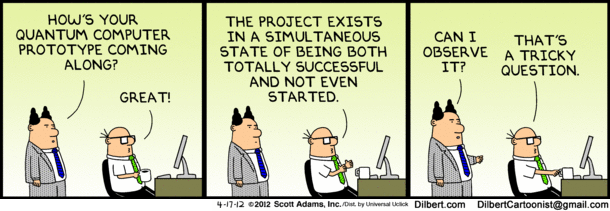
\includegraphics[width=\hsize]{images/dilbert.png}
\caption{Quanten-Computer-Projekt bei Dilbert in einem quantenmechanischen
"Uberlagerungszustand, mit besonderer Ber"ucksichtigung der Wirkung einer
Beobachtung.
\label{skript:dilbert}}
\end{figure}
Nach dem einf"uhrenden Beispiel "uber den Schr"odingerschen
Katzen-Quanten-Computer k"onnen wir uns jetzt dar"uber Gedanken
machen, wie ein Quanten-Computer aussehen m"usste, der allgemeine
mathematische Probleme l"osen k"onnte.
Ein solcher Computer existiert noch nicht, aber ein grosse Zahl von 
Forschungsgruppen (siehe auch Abbildung~\ref{skript:dilbert})
arbeiten daran, die nachstehenden Ideen auf die eine
oder andere Art umzusetzen.

Ein Quantencomputer muss zun"achst einen geeignet komplexen
"Uberlagerungszustand pr"aprieren, den Qubits. Dann muss dieser Zustand
von einem oder mehreren Quanten-Gattern verarbeitet werden, sie
entsprechen dem Operator $Q$ im Schr"odinger-Katzen-Computer.
Schliesslich muss man das Experiment mehrmals durchf"uhren, bis man
Wahrscheinlichkeiten mit gen"ugend grosser Genauigkeit bestimmt hat,
dass man ein Resultat der Berechnung daraus ableiten kann.

Ein solcher Computer bestimmt also mit beschr"ankter Wahrscheinlichkeit
in polynomieller Zeit eine L"osung f"ur ein Problem. Die
Klasse der Probleme, die sich mit beschr"ankter Wahrscheinlichkeit in
polynomieller Zeit auf einem Quantencomputer l"osen lassen, nennen wir
BQP.
Es ist klar, dass $\text{BPP}\subset\text{BQP}$.
\index{BQP, Komplexit\"atsklasse}
\index{Komplexit\"atsklasse!BQP}
Es besteht also die Hoffnung, dass sich in der Klasse BQP Probleme finden,
die ein klassischer Computer auch mit einem probabilistischen Algorithmus
nicht in polynomieller Zeit l"osen kann.

\subsection{Qubits}
Ein quantenmechanisches System mit zwei m"oglichen Zust"ande $|0\rangle$
und $|1\rangle$ muss sich nicht
notwendigerweise in genau einem der Zust"ande befinden.
Jede Linearkombination der beiden Zust"ande ist ebenfalls ein g"ultiger
Zustand, sofern sie als Vektor L"ange $1$ hat.
Der Zustand
\[
|\psi\rangle
=
\lambda \,|0\rangle + \mu\,|1\rangle
\]
hat L"ange $1$, wenn gilt
\[
\langle\psi|\psi\rangle
=
(
\bar\lambda
\langle 0|
+
\bar\mu
\langle 1|
)
(
\lambda \,|0\rangle + \mu\,|1\rangle
)
=
|\lambda|^2\langle 0|0\rangle + |\mu|^2\langle 1|1\rangle
=
|\lambda|^2+|\mu|^2
=
1
,
\]
da die gemischten Terme wegen $\langle 0|1\rangle=0$ wegfallen.
Es gen"ugt also, dass die Quadratsumme der Betr"age von $\lambda$ und $\mu$
den Wert $1$ ergibt.
Insbesondere gibt es selbst f"ur dieses einfache System bereits viel
mehr m"ogliche Zust"ande als bei einem klassischen Bit.
Ein solches quantenmechanisches System nennt man in Qubit.

Ein klassisches System mit zwei Bits kann in 4 m"oglichen Zust"anden sein.
Das zugeh"orige quantenmechanische System kann in einer beliebigen
"Uberlagerung der vier m"oglichen reinen Zust"ande sein:
\[
|\psi\rangle
=
\alpha_{00}|00\rangle
+
\alpha_{01}|01\rangle
+
\alpha_{10}|10\rangle
+
\alpha_{11}|11\rangle
,\qquad
|\alpha_{00}|^2
+
|\alpha_{01}|^2
+
|\alpha_{10}|^2
+
|\alpha_{11}|^2
=1.
\]
Wir nennen dies ein ``2-Qubit Register''.

Praktisch n"utzliche Quantencomputer m"ussen noch wesentlich gr"ossere
Qubits verarbeiten k"onnen.
Ein Register mit $n$ Qubits ist in einem Zustand, in dem $2^n$ Zust"ande
"uberlagert sind.

Es ist auch denkbar, dass wir beim Initialisieren eines Qubits
einzelne auf einen bestimmten Wert setzen.
Zum Beispiel k"onnen wir in einem Register mit $2$ Qubits das erste
Qubit auf $0$ setzen, wir erhalten dann einen Zustand der
Form
\[
|\psi\rangle
=
\alpha_{00}|00\rangle
+
\alpha_{01}|01\rangle
\]
Wir nennen das erste Bit ein Scratch-Bit.
\index{Scratch-bit}

\index{Tensor-Produkt}
Die Operation, aus einzelnen Qubits ein Register von Qubits zu
machen, ist so grundlegend, dass wir daf"ur eine eigene Notation
verwenden wollen.
Sind $H_1$ und $H_2$ die Hilbertr"aume, in denen die Zust"ande f"ur
die einzelnen Bits zu finden sind, dann schreiben wir $H_1\otimes H_2$
f"ur den Raum, der die kombinierten Zust"ande enth"alt.
Sind $|a\rangle\in H_1$ und $|b\rangle\in H_2$ Zust"ande einzelner
Qubits, dann schreiben wir f"ur den kombinierten Zustand auch
$|ab\rangle=|a\rangle\,|b\rangle=|a\rangle\otimes|b\rangle=|a\otimes b\rangle$.
Das Skalarprodukt in $H_1\otimes H_2$ ist gegeben durch
\[
\langle a\otimes b|c\otimes d\rangle
=
\langle a|c\rangle\,\langle b|d\rangle.
\]
Die Zust"ande $|0\otimes 0\rangle$,
$|0\otimes 1\rangle$,
$|1\otimes 0\rangle$ und
$|1\otimes 1\rangle$ sind dann immer noch orthogonal.

\begin{beispiel}
Man berechne das Skalarprodukt der beiden Zust"ande
\[
|\psi\rangle
=
\frac1{\sqrt{2}} |0\rangle\otimes|1\rangle
+
\frac1{\sqrt{2}} |1\rangle\otimes|0\rangle
\qquad
\text{und}
\qquad
|\varphi\rangle
=
\alpha |0\rangle\otimes|1\rangle
+
\beta |1\rangle\otimes|0\rangle.
\]
Wir k"onnen verwenden, dass die Basisvektoren $|a\otimes b\rangle$ orthogonal
sind, und schliessen, dass das Skalarprodukt
$\frac1{\sqrt{2}}\alpha + \frac1{\sqrt{2}}\beta$ sein muss.
Wir wollen uns aber "uberzeugen, dass die Definitionen ``funktionieren''
und rechnen daher das Skalarprodukt auch explizit aus.
Nach Definition des Skalarproduktes in $H_1\otimes H_2$ gilt
\begin{align*}
\langle\psi|\varphi\rangle
&=
\biggl(
\frac1{\sqrt{2}} \langle 0 \otimes 1|
+
\frac1{\sqrt{2}} \langle 1\otimes0|
\biggr)
\biggl(
\alpha |0\otimes 1\rangle
+
\beta |1\otimes 0\rangle.
\biggr)
\\
&=
\frac1{\sqrt{2}} \alpha\langle 0\otimes 1|0\otimes 1\rangle
+
\frac1{\sqrt{2}} \beta \langle 0\otimes 1|1\otimes 0\rangle
+
\frac1{\sqrt{2}} \alpha\langle 1\otimes 0|0\otimes 1\rangle
+
\frac1{\sqrt{2}} \beta \langle 1\otimes 0|1\otimes 0\rangle
\\
&=
\frac1{\sqrt{2}} \alpha\underbrace{\langle 0|0\rangle}_{=1} \underbrace{\langle 1|1\rangle}_{=1}
+
\frac1{\sqrt{2}} \beta \underbrace{\langle 0|1\rangle}_{=0} \underbrace{\langle 1|0\rangle}_{=0}
+
\frac1{\sqrt{2}} \alpha\underbrace{\langle 1|0\rangle}_{=0} \underbrace{\langle 0|1\rangle}_{=0}
+
\frac1{\sqrt{2}} \beta \underbrace{\langle 1|1\rangle}_{=1} \underbrace{\langle 0|0\rangle}_{=1}
\\
&=
\frac1{\sqrt{2}}\alpha + \frac1{\sqrt{2}}\beta,
\end{align*}
wir erhalten also genau das erwartete Resultat.
\end{beispiel}

\subsection{Gatter}
Klassische Computer f"uhren ihre Berechnung mit logischen Gattern durch,
die auf einem Vektor von Bits wirken.
Quantencomputer brauchen Quanten-Gatter, welche auf einem
$n$ Qubit Zustand wirken.
Solche Gatter d"urfen selbst keine Messungen machen, den die
Auswertung der Berechnung darf ja erst ganz am Ende der
Transformationen erfolgen.
Die Gatter sind also Zustands"anderungen, die umkehrbar sein m"ussen.
Eine physikalische Realisierung eines Gatters ist nichts anderes
als eine Zeitentwicklung des urspr"unglichen Zustands durch einen
speziellen Hamilton-Operator.

\begin{definition}
\index{Gatter!Quanten-}
Ein Quanten-Gatter ist ein unit"arer Operator, der auf einem 
$n$-Qubit Zustand operiert.
\end{definition}

\begin{beispiel}
\index{Flip}
\index{Gatter!Flip}
Die {\em Flip Operation} implementiert die Negation eines einzelne Qubit:
\begin{align*}
|0\rangle&\mapsto |1\rangle & |1\rangle&\mapsto |0\rangle.
\end{align*}
Die zugeh"orige Matrix ist
\[
F=\begin{pmatrix}
0&1\\
1&0
\end{pmatrix}.
\]
$F$ ist eine unit"are Matrix, als ein Quanten-Gatter.
\end{beispiel}

\begin{beispiel}
\index{Bit-Umordnung}
\index{Gatter!Bit-Umordnung}
Die {\em Bit-Umordnung} vertauscht zwei Qubits, d.~h.~sie implementiert
die Abbildung:
\begin{align*}
|00\rangle&\mapsto |00\rangle\\
|01\rangle&\mapsto |10\rangle\\
|10\rangle&\mapsto |01\rangle\\
|11\rangle&\mapsto |11\rangle
\end{align*}
Die zugeh"orige Matrix ist
\[
X=
\begin{pmatrix}
1&0&0&0\\
0&0&1&0\\
0&1&0&0\\
0&0&0&1
\end{pmatrix}.
\]
Die Matrix $X$ ist unit"ar, weil orthogonal.
\end{beispiel}

\begin{beispiel}
\index{Phasenshift}
\index{Gatter!Phasenshift}
{\em Phasenshift} ist eine Operation, die den Zust"and $|1\rangle$ 
mit einem Phasenfaktor versieht:
\begin{align*}
|0\rangle &\mapsto |0\rangle\\
|1\rangle &\mapsto e^{i\varphi}\,|1\rangle
\end{align*}
Die zugeh"orige Matrix ist
\[
\begin{pmatrix}
1&0\\
0&e^{i\varphi}
\end{pmatrix},
\]
die Matrix ist nicht orthogonal, aber unit"ar.
\end{beispiel}

\begin{beispiel}
\index{Hadamard}
\index{Gatter!Hadamard}
Die {\em Hadamard-Operation} implementiert eine lineare Abbildung
\begin{align*}
|0\rangle &\mapsto |0\rangle + |1\rangle\\
|1\rangle &\mapsto |0\rangle - |1\rangle,
\end{align*}
wobei die Vektoren auf der rechten Seite noch normiert werden m"ussen.
Die zugeh"orige Matrix ist
\begin{equation}
H=
\frac1{\sqrt{2}}
\begin{pmatrix}
1&\phantom{1}1\\
1&-1
\end{pmatrix}.
\label{skript:hadamard}
\end{equation}
Die Matrix $H$ ist orthogonal, also insbesondere auch unit"ar.
\end{beispiel}

\begin{beispiel}
\index{Gatter!UND}
\index{Gatter!ODER}
Es gibt weder ein UND- noch ein ODER-Gatter f"ur Quantencomputer.
Ein UND-Gatter m"usste die Abbildung
\begin{align*}
|00\rangle&\mapsto|00\rangle,\\
|01\rangle&\mapsto|00\rangle,\\
|10\rangle&\mapsto|00\rangle,\\
|11\rangle&\mapsto|01\rangle
\end{align*}
implementieren, welche nicht invertierbar ist, und daher auch nicht
unit"ar sein kann.
Selbst wenn man die Operationen UND und ODER in eine einzige Abbildung
kombiniert, erh"alt man
\begin{align*}
|00\rangle&\mapsto|00\rangle,\\
|01\rangle&\mapsto|10\rangle,\\
|10\rangle&\mapsto|10\rangle,\\
|11\rangle&\mapsto|11\rangle
\end{align*}
was immer noch nicht invertierbar ist, denn man kann aus den Resultatbits
nicht mehr schliessen, welches der beiden Bits gesetzt war.
Als letzte Hoffnung k"onnten wir versuchen, eines der Bits zu behalten,
aber das funktioniert auch nicht:
\begin{align*}
|00\rangle&\mapsto|00\rangle,\\
|01\rangle&\mapsto|00\rangle,\\
|10\rangle&\mapsto|10\rangle,\\
|11\rangle&\mapsto|11\rangle,
\end{align*}
immer noch nicht invertierbar.
\end{beispiel}

\begin{beispiel}
\index{CNOT-Gatter}
\index{Gatter!CNOT}
Das \textsc{CNOT}-Gatter invertiert das zweite Bit, wenn das erste Bit
gesetzt ist.
Es implementiert also die Abbildung
\begin{align*}
|00\rangle&\mapsto|00\rangle,\\
|01\rangle&\mapsto|01\rangle,\\
|10\rangle&\mapsto|11\rangle,\\
|11\rangle&\mapsto|10\rangle
\end{align*}
Die zugeh"orige Matrix ist
\[
U_{\textsc{CNOT}}=\begin{pmatrix}
1&0&0&0\\
0&1&0&0\\
0&0&0&1\\
0&0&1&0
\end{pmatrix}.
\]
Diese Matrix ist offensichtlich unit"ar.
Manchmal wird das \textsc{CNOT}-Gatter mit dem Diagramm
\begin{center}
\includegraphics{graphics/gatter-10.pdf}
\end{center}
dargestellt werden.
Man beachtet, dass dieses Diagramm im Gegensatz zu den Analysator-Diagrammen
von Kapitel~\ref{chapter:einfache-quantensysteme} von links nach rechts
gelesen werden muss.
\end{beispiel}

\begin{beispiel}
\index{Tofoli-Gatter}
\index{Gatter!Tofoli}
Das {\em Tofoli-Gatter} operiert auf zwei Qubits $a$ und $b$ und einem
Scratch-Bit $c$ und implementiert die Abbildung
\[
|a\otimes b\otimes c\rangle
\mapsto
|a\rangle\otimes|b\rangle\otimes|(a\wedge b)\oplus c\rangle.
\]
Darin ist $\oplus$ die XOR-Operation. 
Im Detail beschreibt dies folgende Abbildung
\begin{align*}
|000\rangle&\mapsto|000\rangle\\
|001\rangle&\mapsto|001\rangle\\
|010\rangle&\mapsto|010\rangle\\
|011\rangle&\mapsto|011\rangle\\
|100\rangle&\mapsto|100\rangle\\
|101\rangle&\mapsto|101\rangle\\
|110\rangle&\mapsto|111\rangle\\
|111\rangle&\mapsto|110\rangle
\end{align*}
In dieser Reihenfolge der Basisvektoren geh"ort dazu die Matrix
\[
T=
\begin{pmatrix}
1&0&0&0&0&0&0&0\\
0&1&0&0&0&0&0&0\\
0&0&1&0&0&0&0&0\\
0&0&0&1&0&0&0&0\\
0&0&0&0&1&0&0&0\\
0&0&0&0&0&1&0&0\\
0&0&0&0&0&0&0&1\\
0&0&0&0&0&0&1&0\\
\end{pmatrix}.
\]
Die Matrix $T$ ist orthogonal, und damit auch unit"ar.
Das Tofoli-Gatter wird manchmal auch als Diagramm
\begin{center}
\includegraphics{graphics/gatter-11.pdf}
\end{center}
dargestellt. Das Zeichen \textsc{AND} erinnert daran, dass das Tofoli-Gatter
eigenlicht die UND-Verkn"upfung der beiden Inputs $a$ und $b$ berechnet.
\end{beispiel}

\begin{beispiel}
\begin{figure}
\centering
\includegraphics{graphics/gatter-12.pdf}
\caption{Implementation eines \textsc{CNOT}-Gatters aus einem Tofoli-Gatter
mit Hilfe eines Scratch-Bit \label{skript:cnot=tofoli}}
\end{figure}
Man kann aus einem Tofoli-Gatter mit Hilfe eines Scratch-Bit ein
\textsc{CNOT}-Gatter machen, wie in Abbildung~\ref{skript:cnot=tofoli}
dargestellt.
\end{beispiel}

\subsection{Die Hadamard-Operation}
Die Hadamard-Operation (\ref{skript:hadamard}) auf einem einzelnen
Qubit wird durch die Matrix
\[
H=
\frac{1}{\sqrt{2}}\begin{pmatrix}1&1\\1&-1\end{pmatrix}
\]
gegeben.
Die Wirkung von $H$ auf einem einzelnen Qubit $|x\rangle$ ergibt die Summe oder
Differenz von $|0\rangle$ und $|1\rangle$, je nachdem ob $x=0$ oder $x=1$.
Man kann dies auch durch
\[
H\,|x\rangle = \frac1{\sqrt{2}}(|0\rangle + (-1)^x|1\rangle)
\]
ausdr"ucken.

Auf einem $n$-Qubit-Register $|x\rangle$ wirkt $H^{\otimes n}$ bitweise.
F"ur ein $2$-Qubit-Register bedeutet dies
\begin{align*}
|x_1\rangle \otimes |x_2\rangle
&\mapsto
\frac1{\sqrt{2}} \biggl( |0\rangle + (-1)^{x_1}|1\rangle \biggr)
\frac1{\sqrt{2}} \biggl( |0\rangle + (-1)^{x_2}|1\rangle \biggr)
\\
&=
\frac12(
|00\rangle
+
(-1)^{x_1}
|10\rangle
+
(-1)^{x_2}
|01\rangle
+
(-1)^{x_1+x_2}
|11\rangle
)
\\
&=
\frac12
\sum_{y} (-1)^{x\cdot y} |y\rangle.
\end{align*}
Die zugeh"orige unit"are Matrix in der Basis
$\{|00\rangle,
|10\rangle,
|01\rangle,
|11\rangle\}$
ist
\[
H^{\otimes 2}
=
\frac12
\begin{pmatrix}
 1& 1& 1& 1\\
 1&-1& 1&-1\\
 1& 1&-1&-1\\
 1&-1&-1& 1
\end{pmatrix}.
\]
Es ist offensichtlich, dass die Zeilen und Spalten orthonormiert sind,
wie man das f"ur eine unit"are Matrix erwartet.
Ausserdem pr"uft man leicht nach, dass $H^{\otimes 2}\cdot H^{\otimes 2}=E$.

F"ur ein $n$-Qubit-Register $|x\rangle$ gilt analog
\begin{align*}
H^{\otimes n}\, |x\rangle
=
\frac1{(\sqrt{2})^n}
\sum_y (-1)^{x\cdot y}|y\rangle
\end{align*}
Das Resultat der Hadamard-Operation ist also ein Zustand, in dem
jeder m"ogliche reine Zustand mit gleicher Wahrscheinlichkeit vertreten ist.
Das Vorzeichen von $|y\rangle$ in $H^{\otimes n}|x\rangle$ ist
$(-1)^{x\cdot y}$.

\subsection{No-Cloning Theorem}
Ein klassischer Computer kann ein Ausgangssignal als Input f"ur viele
nachfolgende Gatter verwenden, das Bit wird einfach auf mehrere Leitungen
kopiert. 
Ein Quanten-Computer kann das nicht:
\begin{satz}
\label{skript:no-cloning-theorem}
Es gibt keine unit"are Matrix, die einen beliebigen Zustand kopieren
kann, d.~h.~die Abbildung
\[
|\psi\rangle\otimes|k\rangle\mapsto |\psi\rangle\otimes|\psi\rangle
\]
kann nicht unit"ar sein.
\end{satz}

\begin{proof}[Beweis]
Nehmen wir an, es g"abe eine unit"are Abbildung $U$, die ein Qubit clonen
kann:
\[
U(|\psi\rangle\otimes k\rangle)=|\psi\rangle\otimes\psi\rangle.
\]
Wenden wir $U$ auf einen analog konstruierten Zustand
$|\varphi\rangle\otimes k\rangle$ an, dann muss, weil $U$ unit"ar ist,
das Skalarprodukt der beiden Zust"ande vor und nach der Anwendung
von $U$ gleich sein.
\begin{equation}
\left.
\begin{aligned}
\langle\varphi\otimes k|\psi\otimes k\rangle
&=
\langle\varphi|\psi\rangle \langle k|k\rangle
\\
\langle\varphi\otimes\varphi|\psi\otimes\psi\rangle
&=
\langle\varphi|\psi\rangle \langle \varphi|\psi\rangle
\end{aligned}
\quad
\right\}=
\end{equation}
Da $\langle k|k\rangle=1$ ist, folgt
\[
\langle \varphi|\psi\rangle^2=
\langle \varphi|\psi\rangle
\qquad\Leftrightarrow\qquad
\langle \varphi|\psi\rangle ( \langle \varphi|\psi\rangle -1) = 0
\qquad\Leftrightarrow\qquad
\langle \varphi|\psi\rangle =\begin{cases}0\\1\end{cases}
\]
Die beiden Zust"ande $|\psi\rangle$ und $|\varphi\rangle$ waren aber
beliebig, k"onnen also auch beliebige komplexe Zahlen als Skalarprodukt
haben.
Dieser Widerspruch zeigt, dass es eine solche Matrix $U$ gar nicht
geben kann.
\end{proof}

Qubits lassen sich also grunds"atzlich nicht kopieren.
Dies wird in der Quanten-Kryptographie zur Absicherung des
Schl"usselaustausches verwendet. 
Da der Quantenzustand, den ein Teilnehmer empf"angt, nicht kopiert
werden kann, ist es unm"oglich, den Schl"usselaustausch abzuh"oren,
ohne dass dies bemerkt wird.

\subsection{Quanten-Turing-Maschinen}
Eine Quanten-Berechnung stellt also zuerst einen Zustand in einem
Qubit-Register her.
Dann operiert darauf eine Quantenoperation, also ein unit"arer Operator $U$.
Zum Schluss finden Messungen an den einzelnen Qubits statt.
Das Resultat der Messung verr"at etwas "uber das Resultat der Berechnung.

Um einen Quantencomputer zu realisieren muss man also eine Methode
entwickeln, einen beliebigen Operator $U$ herzustellen.
In einem klassischen Computer geschieht das durch Verschaltung der
Gatter: jede beliebige logische Formal kann aus den elementaren
Gattern hergestellt werden.
F"ur Quantencomputer geht das nicht mehr exakt, das ist aber auch nicht
n"otig, wir sind ohnehin nur auf eine Approximation aus.

\begin{satz}
Jede unit"are $n\times n$-Matrix $U$ mit $n\ge 3$ kann beliebig genau
approximiert werden durch ein Produkt $U_l\dots U_1$ von unit"aren
Matrizen, die jeweils Hadamard-Gatter, Tofoli-Gatter oder Phasen-Shifts
sind.
\cite[Theorem 10.12]{skript:arorabarak}
\end{satz}

\subsection{Quanten-Algorithmen}
Als Beispiel eines Quanten-Algorithmus untersuchen wir den Algorithmus
von Grover:
\begin{satz}[Grover]
Es gibt einen Quantenalgorithmus, der zu einer in polynomieller Zeit
berechenbaren Funktion $f\colon\{0,1\}^n\to\{0,1\}$ einen String von Bits
$a\in\{0,1\}^n$ findet, so dass $f(a)=1$, wenn es einen solchen String gibt.
Die Laufzeit des Algorithmus ist $p(n) 2^{\frac{n}2}$, wobei $p(n)$ ein
Polynom ist.
\label{skript:satz-von-grover}
\end{satz}

Das Problem, welches der Algorithmus von Grover l"ost, erinnert an das
Problem SAT.
Dort wird gefragt, ob in einer logischen Formel $\varphi$ die Variablen
so mit Wahrheitswerten belegt werden k"onnen, dass die Formel wahr wird.
Eine logische Formel ist eine Abbildung $\varphi\colon\{0,1\}^n\to\{0,1\}$,
in SAT wird also gefragt, ob es einen Bit-String $a\in\{0,1\}^n$ gibt, 
so dass $\varphi(a)=1$ ist.
Der Algorithmus von Grover l"ost also SAT.

Wenn man SAT durch Durchprobieren l"osen will, braucht man daf"ur $2^n$
Versuche, die Laufzeit ist exponentiell.
Der Algorithmus von Grover hat zwar auch immer noch exponentielle Laufzeit,
aber der Exponent ist halb so gross.
Daraus sch"opfen die Quantencomputer-Forscher die Hoffnung, dass 
ein Quantencomputer einige Probleme wird l"osen k"onnen, die mit
klassischen Computern nicht l"osbar sind.

\begin{proof}[Beweisidee]
Es geht darum, einen Vektor $|a\rangle$ zu finden, f"ur den $f(a)=1$.
Wir nehmen der Einfachheit halber an, dass es nur eine einzige L"osung $a$
gibt.
Man kann n"amlich schon mit klassischen Mitteln zeigen, dass sich das
Problem immer auf diesen Spezialfall reduzieren l"asst.
Im folgenden bezeichnen wir mit $|y\rangle$ immer einen Zustand mit
$y\in\{0,1\}^n$ aber $y\ne a$.

Zun"achst m"ussen wir aus $f$ eine unit"are Transformation machen.
Wir nehmen das Tofoli-Gatter als Vorbild, und betrachten die Abbildung
\[
|x s\rangle \mapsto |x (s\oplus f(x))\rangle.
\]
Es gibt im Wesentlichen die folgenden vier F"alle
\begin{align*}
|a0\rangle&\mapsto |a1\rangle\\
|a1\rangle&\mapsto |a0\rangle\\
|y0\rangle&\mapsto |y0\rangle\\
|y1\rangle&\mapsto |y1\rangle
\end{align*}
Wir k"onnen das auch symbolisch durch die Matrix
\[
U_f
=
\begin{pmatrix}
0&1&0&0\\
1&0&0&0\\
0&0&1&0\\
0&0&0&1
\end{pmatrix}
\]
darstellen. Es ist offensichtlich, dass diese Operation unit"ar ist, 
wir d"urfen also annehmen, dass wir sie mit einem Quantencomputer
implementieren k"onnen.

Um $a$ zu finden, m"ussen wir jetzt eine Folge von Quantenoperationen
finden, die aus einem bekannten Zustand den Zustand $|a\rangle$ herstellt.
Die Quantenoperationen sind unit"are Operatoren, die wir uns als Drehungen
in einem komplexen Vektorraum vorstellen k"onnen.
Wir k"onnen daher unsere geometrische Intuition verwenden, um die Drehungen
zu finden.

Als Ausgangsvektor verwenden wir einen vollst"andig verschr"ankten Zustand
\[
u=\frac1{\sqrt{2^n}}\sum_{x\in\{0,1\}^n}|x\rangle
\]
in einem $n$-Qubit-Register.
Der Winkel zwischen $|a\rangle$ und $u$ ist
\[
\cos\vartheta
=
\langle u|a\rangle
=
\frac1{\sqrt{2^n}}
\sum_{x\in\{0,1\}^n}\langle x|a\rangle
=
\frac1{\sqrt{2^n}}.
\]
F"ur grosses $n$ ist die rechte Seite nahe bei $0$, der Winkel ist
also nahe bei einem rechten.
Er unterscheidet sich von einem rechten Winkel um
$\sin\vartheta=1/{\sqrt{2^n}}$.
F"ur grosses $n$ ist $\vartheta\simeq 1/{\sqrt{2^n}}$.

Wir suchen jetzt eine Folge von Drehungen, und damit
eine Folge von Vektoren $w_1$, $w_2$, \dots, die den Vektor $u$ sukzessive
immer n"aher an $a$ herandreht.
Wir m"ochten, dass der Winkel zwischen $w_i$ und $a$ in jedem Schritt 
um $\vartheta$ kleiner wird.
Um den Vektor $a$ zu erreichen, brauchen wir also eine Anzahl Schritte
in der Gr"ossenordnung von $O(1/\vartheta)=O(\sqrt{2^n})$.

Um dies durchzuf"uhren m"ussen wir jetzt also nur noch die Drehungen
konstruieren, die den Winkel zu $a$ kleiner machen.
Dies m"ussen wir schaffen ohne die Kenntnis von $a$, und es muss mit
einer Quantenoperation implementiert werden k"onnen.
\end{proof}

\begin{hilfssatz}
Der Vektor
\[
e=\sum_{y\ne a}|y\rangle
\]
steht senkrecht auf $a$.
Der Winkel zwischen $u$ und $e$ ist $\vartheta$.
\label{skript:hilfssatz-winkel}
\end{hilfssatz}

\begin{proof}[Beweis]
Wir rechnen das Skalarprodukt aus
\[
\langle a|e\rangle
=
\sum_{y\ne a}\langle a|y\rangle =0.
\]
Der Winkel $\vartheta$ war definiert als der Komplementwinkel
des Winkels zwischen $a$ und $u$.
Da $a$ senkrecht steht auf $e$, ist das auch der Winkel zwischen
$e$ und $a$.
\end{proof}

\begin{hilfssatz}
Seien $\vec v_1$ und $\vec v_2$ zwei Vektoren in einer Ebene
$\sigma\subset V$, und sei $\alpha$ der Winkel zwischen $\vec v_1$
und $\vec v_2$.
Die an der Achse $\vec v_1$ und gefolgt von der Spiegelung an der Achse
$\vec v_2$ ist eine Drehung in der Ebene $\sigma$ um den Winkel $2\alpha$,
die alle Vektoren senkrecht dazu unver"andert l"asst.
\label{skript:hilfssatz-drehung}
\end{hilfssatz}

\begin{proof}[Beweis]
\begin{figure}
\centering
\includegraphics{graphics/gatter-13.pdf}
\caption{Spiegelung an der Achse $\vec v_1$ bildet $\vec w$ auf $\vec w'$ ab.
\label{skript:drehung-spiegelung-1}}
\end{figure}
\begin{figure}
\centering
\includegraphics{graphics/gatter-14.pdf}
\caption{Spiegelung an der Achse $\vec v_2$ bildet $\vec w'$ auf $\vec w''$ ab.
\label{skript:drehung-spiegelung-2}}
\end{figure}
Die beiden Spiegelungen sind in den Abbildung
\ref{skript:drehung-spiegelung-1}
und
\ref{skript:drehung-spiegelung-2}
dargestellt.
Die Zeichenebene ist $\sigma$ mit den Vektoren $\vec v_1$ und $\vec v_2$.
Man kann unmittelbar aus der Zeichnung ablesen, dass
die Abbildung $\vec w\mapsto \vec w''$ eine Drehung im $2\vartheta$ ist.
\end{proof}

\begin{hilfssatz}
Die Spiegelung an $e$ gefolgt von einer Spiegelung an $u$ 
ist eine Drehung $R$ um $2\vartheta$ in der von $|a\rangle$ und $u$
aufgespannten Ebene.
\label{skript:hilfssatz-schritt}
\end{hilfssatz}

\begin{proof}
Zun"achst ist nach Hilfssatz~\label{skript:hilfssatz-winkel}
der Winkel zwischen $u$ und $e$ gleich $\vartheta$.
Nach Hilfssatz~\ref{skript:hilfssatz-drehung} ist die Spiegelung
an $u$ gefolgt von einer Spiegelung an $e$ eine Drehung in der
von $a$ und $u$ aufgespannten Ebene um den Winkel $2\vartheta$.
\end{proof}

\begin{hilfssatz}
Die Spiegelung eines Vektors $w$ in der $u$-$a$-Ebene an
der Achse $e$ kann mit einer Quantenoperation durchgef"uhrt werden.
\label{skript:hilfssatz-spiegelung-e}
\end{hilfssatz}

\begin{proof}[Beweis]
Um die Spiegelung eines Vektors $\vec w$ an der Achse $e$ durchzuf"uhren,
m"ussen wir den Vektor in Komponenten parallel zu $e$ und senkrecht
auf $e$ zerlegen, und das Vorzeichen der Komponenten senkrecht auf
$e$ umkehren.
Wir brauchen also eine Abbildung der Form
\begin{align*}
|a\rangle&\mapsto -|a\rangle\\
|y\rangle&\mapsto \phantom{-}|y\rangle.
\end{align*}
Dazu brauchen wir zus"atzlich eine Abbildung mit Matrix
\[
Z=\begin{pmatrix}
1&0\\0&-1
\end{pmatrix},
\]
die wir auf ein Scratch-Bit wirken lassen.
Wir setzen sie mit $U_f$ zusammen:
\begin{equation}
\begin{tabular}{
>{$}l<{$}
>{$}c<{$}
>{$}l<{$}
>{$}c<{$}
>{$}l<{$}
>{$}c<{$}
>{$}l<{$}
}
          &Z      &                     &U_f    &                     &Z      &                     \\
|a0\rangle&\mapsto&\phantom{-}|a0\rangle&\mapsto&\phantom{-}|a1\rangle&\mapsto&         - |a1\rangle\\
|a1\rangle&\mapsto&         - |a1\rangle&\mapsto&         - |a0\rangle&\mapsto&         - |a0\rangle\\
|y0\rangle&\mapsto&\phantom{-}|y0\rangle&\mapsto&\phantom{-}|y0\rangle&\mapsto&\phantom{-}|y0\rangle\\
|y1\rangle&\mapsto&         - |y1\rangle&\mapsto&         - |y1\rangle&\mapsto&\phantom{-}|y1\rangle
\end{tabular}
\end{equation}
Ignoriert man das Scratch-Bit, haben wir tats"achlich eine Abbildung realisiert,
die genau die $|a\rangle$-Komponente umkehrt.
\end{proof}

\begin{hilfssatz}
Die Spiegelung an der Achse $u$ kann mit einer Quantenoperation
durchgef"uhrt werden.
\label{skript:hilfssatz-spiegelung-u}
\end{hilfssatz}

\begin{proof}[Beweis]
Wir wenden zuerst die Hadamard-Operation $H$ auf jedes Bit an.
Dabei wird aus $u$ der Vektor $|0\dots 0\rangle$.
Dazu berechnen wir die Wirkung von $H$ auf einem Zustand $u$:
\begin{align*}
Hu
&=
\frac1{\sqrt{2^n}}\sum_{x'\in\{0,1\}^{n-1}}(H\,|0x'\rangle + H\,|1x'\rangle)
=
\frac1{\sqrt{2}}(H\,|0\rangle + H\,|1\rangle)\otimes
  \frac1{\sqrt{2^{n-1}}}\sum_{x'\in\{0,1\}^{n-1}} |x'\rangle
\\
&=
|0\rangle\otimes
  \frac1{\sqrt{2^{n-1}}}\sum_{x'\in\{0,1\}^{n-1}} |x'\rangle
\end{align*}
Wiederholt man dies f"ur jedes Qubit, entsteht der Vektor $|0\dots 0\rangle$.
Jetzt muss die $|0\rangle$-Komponente umgekehrt werden, was mit der Abbildung
\begin{align*}
|0\dots0\rangle&\mapsto          - |0\dots0\rangle\\
|x\rangle      &\mapsto \phantom{-}|x\rangle,\qquad x\ne 0\dots 0
\end{align*}
geschehen kann, die offensichtlich unit"ar ist.
Danach kehrt man die Hadamard-Abbildung wieder um.
\end{proof}

\begin{proof}[Beweis von Satz~\ref{skript:satz-von-grover}]
Damit l"asst sich der Beweis von Satz~\ref{skript:satz-von-grover}
nun vervollst"andigen.
In der Beweisidee haben wir schon dargelegt, wie der Vektor
$|a\rangle$ aus dem Vektor $|u\rangle$ durch gen"ugend viele
Drehungen um den Winkel $2\vartheta$ entstehen kann.
In Hilfssatz~\ref{skript:hilfssatz-schritt} haben wir gezeigt, dass
die gesuchte Drehung als Zusammensetzung von Spiegelungen realisiert
werden kann.
In den Hilfss"atzen~\ref{skript:hilfssatz-spiegelung-u} und
\ref{skript:hilfssatz-spiegelung-e} schliesslich haben wir gezeigt,
dass beide Spiegelungen Quantenoperationen sind.
Damit ist gezeigt, dass $|a\rangle$ durch Iteration von
Quantenoperationen gefunden werden kann.
\end{proof}

Der Algorithmus von Grover zeigt geometrisch anschaulich, wie der
``zus"atzliche Platz'' im Zustandsraum eines Quantencomputers
die Konstruktion einer L"osung erm"oglich.
Nat"urlich ist die quadratische Beschleunigung im Algorithmus
von Grover nicht berauschend.
Es wurden aber auch Algorithmen mit polynomieller Laufzeit f"ur
SAT-verwandte Probleme gefuden, zum Beispiel der Algorithmus von
Simon.
Vielversprechend ist auch die Tatsache, dass f"ur die Faktorisierung
von Zahlen mit dem Algorithmus von Shor \cite{skript:arorabarak}
ebenfalls ein polynomieller Algorithmus f"ur ein klassisch
nicht polynomielles Problem bekannt ist.

Die Beispiele illustrieren jedoch auch, dass ein n"utzlicher
Quantencomputer "uber eine recht grosse Zahl von Qubits verf"ugen
muss.
F"ur kleine Problemgr"ossen lohnt sich der zus"atzliche Aufwand
eines Quantencomputers nicht.
Quantenalgorithmen sind ja grunds"atzlich probabilistischer
Natur, Resultate sind erst nach vielen Wiederholungen verf"ugbar.
Zum Beispiel l"asst sich SAT f"ur eine Formel mit 32 Variablen
innert Sekunden auf einem klassischen Computer entscheiden.
So grosse Qubit-Register lassen sich heute technisch noch nicht
realisieren.

Sollten einst gen"ugend grosse Qubit-Register zur Verf"ugung
stehen, m"ussen immer noch die Quantenoperationen realisiert
werden.
Dabei besteht immer die Gefahr, dass der sensible verschr"ankte
Quantenzustand zerst"ort wird.
Daher verwenden alle bekannten Ans"atze zum Bau von
Quanten-Computern auf Temperaturen nahe dem absoluten
Nullpunkt gek"uhlte Komponenten, um eine Beeinflussung des
Zustandes durch die thermische Bewegung der Molek"ule
zu beschr"anken.
Bis zur vollst"andigen Realisierung eines Quanten-Computers
ist also noch ein weiter Weg.

\section*{"Ubungsaufgabe}
\rhead{"Ubungsaufgabe}
\begin{uebungsaufgaben}
\item
Ist die Operation
\[
|abc\rangle\mapsto |(a\vee b)\oplus c\rangle
\]
durch ein Quantengatter implementierbar?

\begin{loesung}
Diese Operation beschreibt die Abbildung
\begin{align*}
|000\rangle&\mapsto|000\rangle\\
|001\rangle&\mapsto|001\rangle\\
|010\rangle&\mapsto|011\rangle\\
|011\rangle&\mapsto|010\rangle\\
|100\rangle&\mapsto|101\rangle\\
|101\rangle&\mapsto|100\rangle\\
|110\rangle&\mapsto|111\rangle\\
|111\rangle&\mapsto|110\rangle.
\end{align*}
Dazu geh"ort die Matrix
\[
U
=
\begin{pmatrix}
1&0&0&0&0&0&0&0\\
0&1&0&0&0&0&0&0\\
0&0&0&1&0&0&0&0\\
0&0&1&0&0&0&0&0\\
0&0&0&0&0&1&0&0\\
0&0&0&0&1&0&0&0\\
0&0&0&0&0&0&0&1\\
0&0&0&0&0&0&1&0\\
\end{pmatrix}
\]
Dies ist eine orthogonale Matrix, also ist $U$ ein Quantengatter.
\end{loesung}


\end{uebungsaufgaben}
